\documentclass[psfig,11pt]{article} 
 
\textheight 24.4cm
\textwidth 16.59cm
\topmargin -0.0cm
\oddsidemargin -0.04in
\evensidemargin -0.04in

\def\normalstretch{1.0}
\def\talllinestretch{1.5}
\def\shortlinestretch{0.8}
\renewcommand{\baselinestretch}{\normalstretch}
\parskip 1ex
\renewcommand{\topfraction}{.75}
\renewcommand{\textfraction}{.20}
\renewcommand{\floatsep}{0.0pt}
\renewcommand{\textfloatsep}{1.0cm}
\renewcommand{\floatpagefraction}{.85}

\def\portindent{\hspace{\parindent}}
\newcommand{\REM}[1]{} 
%\newcommand{\sol}[1]{\noindent\textcolor{red}{{#1}}}
%\newcommand{\solspace}[1]{}
\newcommand{\sol}[1]{\REM{#1}}
\newcommand{\solspace}[1]{\vspace{#1}}

\newif\ifsol
%\soltrue

\newcommand{\Bsol}{\ifsol \noindent \color{red}}
\newcommand{\Esol}[1]{\color{black} 
\else 
\vspace{{#1}} 
 \fi
 }

\input epsf
\usepackage{epsfig}
\usepackage{subfigure}
\usepackage{fullpage}
\usepackage{multirow}
%\usepackage{multicolumn}
\pagestyle{plain}
\usepackage[usenames]{color}

\begin{document}

\newcounter{quest}
\newenvironment{question}[1][??]{\noindent{\bf Question  \stepcounter{quest}
\arabic{quest} (\textrm{#1} points): }}

\begin{question}[20] Consider a processor with a 2 GHz clock frequency, and separate instruction and data L1 caches. The base CPI with no memory stalls is 1. The instruction cache has a miss rate of 1\% and the data cache has a miss rate of 4\%. In the program running on this machine, approximately 25\% of the instructions are loads and 15\% are stores. On a cache miss, the processor must stall for 100 {\it ns} to complete a memory access. 

\begin{enumerate}

\item ({\bf 6 marks})   What percentage of the total time spent by the program is memory stalls?

\ifsol
\color{red}
Assume that the program executes 1000 instructions.\\
For the ideal machine (without any misses), the accesses to the data cache happen in parallel with the accesses to the instruction cache. With a 2 GHz clock frequency, the clock cycle is 0.5 {\it ns} Therefore:

\begin{eqnarray}
\mathrm{Optimal\ time} &=& 1000 \mathrm{\ cycles} \times 0.5 \mathit{\ ns} = 500 \mathit{\ ns} \nonumber \\
\mathrm{Actual\ time} &=& \mathrm{hit\ time} + \mathrm{miss\ time} \nonumber \\
\mathrm{Actual\ time} &=& 500 \mathit{\ ns} + (1000 \times 0.01 + 400 \times 0.04) \times 100 \mathit{\ ns} \nonumber \\
\mathrm{Actual\ time} &=& 500 \mathit{\ ns} + 2600 \mathit{\ ns} = 3100 \mathit{\ ns} \nonumber \\
\mathrm{Percentage\ time} &=& \frac{2600}{3100} \times 100 = 84\% \nonumber
\end{eqnarray}

\color{black}
\else
\vspace{1.5in}
\fi

\item ({\bf 6 marks})   What is the average memory access time (in nanoseconds) for this machine?

\ifsol
\color{red}
Even though there are only 1000 cycles to access both instruction and data L1 cache, there are actually 1400 access, thus this number has to be used when computing AMAT

\begin{eqnarray}
\mathrm{AMAT} &=&  \frac{\mathrm{hit\ time} + \mathrm{miss\ rate} \times \mathrm{miss\ penalty}}{\mathrm{\#\ of\ accesses}}  \nonumber \\
&=& \frac{500  \mathit{\ ns} + 2600 \mathit{\ ns}}{1400} = 2.21 \frac{\mathit{ns}}{\mathrm{access}}
\end{eqnarray}

\color{black}
\else
\vspace{1.5in}
\fi

\item ({\bf 8 marks})   To improve performance, your machine is being redesigned to include an L2 unified cache. The L2 cache has an access time of 10 {\it ns}, but will reduce the number of accesses to memory to 1\% of all L1 accesses. How many times faster is this machine than the one in Part (b)? 

\ifsol
\color{red}

See diagram on next page.

\begin{figure}[h!]
\centering
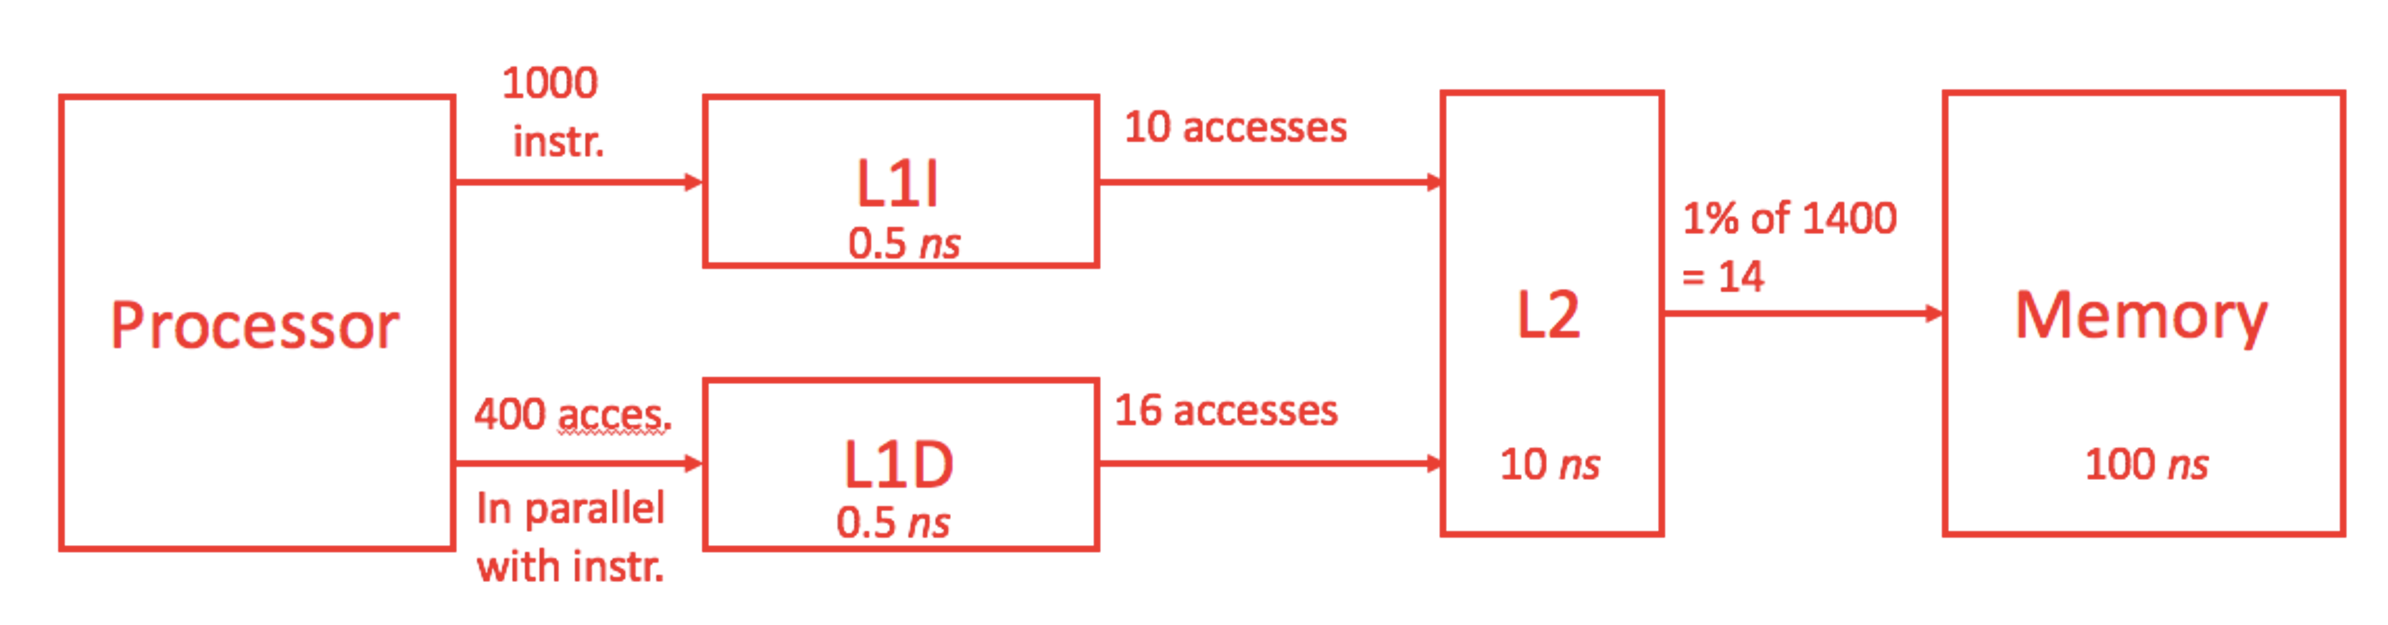
\includegraphics[scale=0.4]{W14-final-Q4-AMAT.pdf}
\end{figure}

\begin{eqnarray}
\mathrm{AMAT} &=&  \frac{1000 \times 0.5  \mathit{\ ns} + 26 \times 10 \mathit{\ ns} + 14 \times 100 \mathit{\ ns} }{1400 \mathrm{\ accesses}} = 2.21 \frac{\mathit{ns}}{\mathrm{access}}  \nonumber \\
&=&  \frac{500  \mathit{\ ns} + 260 \mathit{\ ns} + 1400 \mathit{\ ns} }{1400 \mathrm{\ accesses}} = \frac{2160 \mathit{\ ns}}{1400 \mathrm{\ accesses}} = 1.54 \frac{\mathit{\ ns}}{\mathrm{\ accesses}} \nonumber \\
\mathrm{Speedup} &=& \frac{3100 \mathit{\ ns}}{2160 \mathit{\ ns}} = 1.44 \nonumber
\end{eqnarray}

This machine is 1.44 times faster than the one in Part (b).

\color{black}
\else
\vspace{1.5in}
\fi

\end{enumerate}
\end{question}


\end{document}

